\documentclass[journal]{IEEEtran} % use the `journal` option for ITherm conference style
\IEEEoverridecommandlockouts
% The preceding line is only needed to identify funding in the first footnote. If that is unneeded, please comment it out.
\usepackage{cite}
\usepackage{amsmath,amssymb,amsfonts}
\usepackage{algorithmic}
\usepackage{graphicx}
\usepackage{textcomp}
\usepackage{xcolor}
\usepackage{float} 
\usepackage{hyperref}

% Configuración de hyperref para enlaces en azul
\hypersetup{
    colorlinks=true,
    linkcolor=blue,
    urlcolor=blue,
    citecolor=blue
} 
\def\BibTeX{{\rm B\kern-.05em{\sc i\kern-.025em b}\kern-.08em
    T\kern-.1667em\lower.7ex\hbox{E}\kern-.125emX}}
\begin{document}

\title{ Simulación de Conmutación Telefónica y Análisis de Tráfico \\
% delete or comment-out the following line before submission
%{\footnotesize \textsuperscript{*}Note: Sub-titles are not captured in Xplore and should not be used}
\thanks{Identify applicable funding agency here. If none, delete this.}
}

\author{%%%% author names
    \IEEEauthorblockN{Darwin Cristhian Turpo Quispe}% first author
    , \IEEEauthorblockN{Luque Llanqui Vladimir Williams}% second author
    , \IEEEauthorblockN{Maldonado Lima Roger Jhon}% third author
    % duplicate the line above as many times as needed to list all authors
    \\%%%% author affiliations
    \IEEEauthorblockA{\textit{Escuela Profesional de Ingeniería en Telecomunicaciones}}\\% first affiliation
    \IEEEauthorblockA{\textit{Universidad Nacional de San Agustín de Arequipa}}\\% second affiliation
    \IEEEauthorblockA{\textit{Repositorio: \href{https://github.com/DarwinTQ/lab_sistemas_telefonia/tree/main/lab02}{https://github.com/DarwinTQ/lab\_sistemas\_telefonia/tree/main/lab02}}}\\% repository
    % duplicate the line above as many times as needed to list all affiliations
    %%%% corresponding author contact details
    %\IEEEauthorblockA{email address or ORCID of corresponding author(s)}
}

\maketitle

% \begin{abstract}
%     This document is a model and instructions for \LaTeX.
%     This and the IEEEtran.cls file define the components of your paper [title, text, heads, etc.]. *CRITICAL: Do Not Use Symbols, Special Characters, Footnotes,
%     or Math in Paper Title or Abstract.
% \end{abstract}

% \begin{IEEEkeywords}
%     component, formatting, style, styling, insert
% \end{IEEEkeywords}

\section{Introducción}
El presente laboratorio tiene como objetivo principal simular el funcionamiento de un sistema de conmutación telefónica y analizar su comportamiento bajo carga de tráfico utilizando la teoría de colas y el software Matlab. Se busca modelar una matriz de conmutación, simular el establecimiento y liberación de llamadas, y analizar el fenómeno de bloqueo. A través de la simulación, se calculará la probabilidad de bloqueo y se comparará con los valores teóricos obtenidos mediante la fórmula de Erlang B para validar el modelo. Finalmente, se analizarán parámetros de Calidad de Servicio (QoS) y se realizarán recomendaciones de dimensionamiento de recursos para garantizar un Grado de Servicio (GoS) aceptable.

\section{Marco Teórico}

\subsection{Conmutación de Circuitos}
Sistema donde se establece un camino físico dedicado entre los interlocutores durante toda la llamada:
\begin{itemize}
    \item Matriz de conmutación: $N \times N$ (N líneas)
    \item Probabilidad de bloqueo: $P_b = \frac{A^N/N!}{\sum_{k=0}^{N} A^k/k!}$
\end{itemize}

\subsection{Teoría de Tráfico Telefónico}
\begin{itemize}
    \item Erlang (E): Unidad de intensidad de tráfico
    \item Erlang B: Probabilidad de bloqueo en sistemas con pérdidas
    \item Erlang C: Probabilidad de espera en sistemas con colas
    \item Ley de Little: $L = \lambda W$
\end{itemize}

\subsection{Parámetros de Calidad de Servicio (QoS)}
\begin{itemize}
    \item Grado de Servicio (GoS): Probabilidad de bloqueo aceptable
    \item Utilización: $\rho = \frac{A}{N}$
    \item Retardo promedio: $W = \frac{1}{\mu - \lambda}$
\end{itemize}

\subsection{Dimensionamiento de Recursos}
\begin{itemize}
    \item Líneas necesarias: $N = f(A, P_b)$
    \item Tráfico admitido: $A = f(N, P_b)$
\end{itemize}

\section{Desarrollo}

\subsection{Simulación del Conmutador Telefónico}\label{AA}
Los parámetros iniciales, como una frecuencia de muestreo $f_s=8000$ Hz y una duración de 0.5 segundos por tono.


\subsection{Análisis de Tráfico y Comparación con Erlang B}



\section{Resultados}
\subsection{Simulación del Conmutador Telefónico}\label{AA}

\begin{verbatim}
    === ESTADÍSTICAS DE SIMULACIÓN ===
Total de llamadas generadas: 202
Llamadas completadas: 202
Llamadas bloqueadas: 0
Probabilidad de bloqueo: 0.0000 ( 0.00 %)
Trafico ofrecido: 5.050 Erlangs
Trafico cursado: 5.050 Erlangs
Utilización del sistema: 20.20 % 

\end{verbatim}

La figura 1  muestra ocupacion del sistema en el tiempo. distribuicion de duraciónde llamadas , la probabilidad de bloqueo es 0.0000 (0.00\%) y la utilización del sistema es 20.20\%.
 \begin{figure}[H]
     \centerline{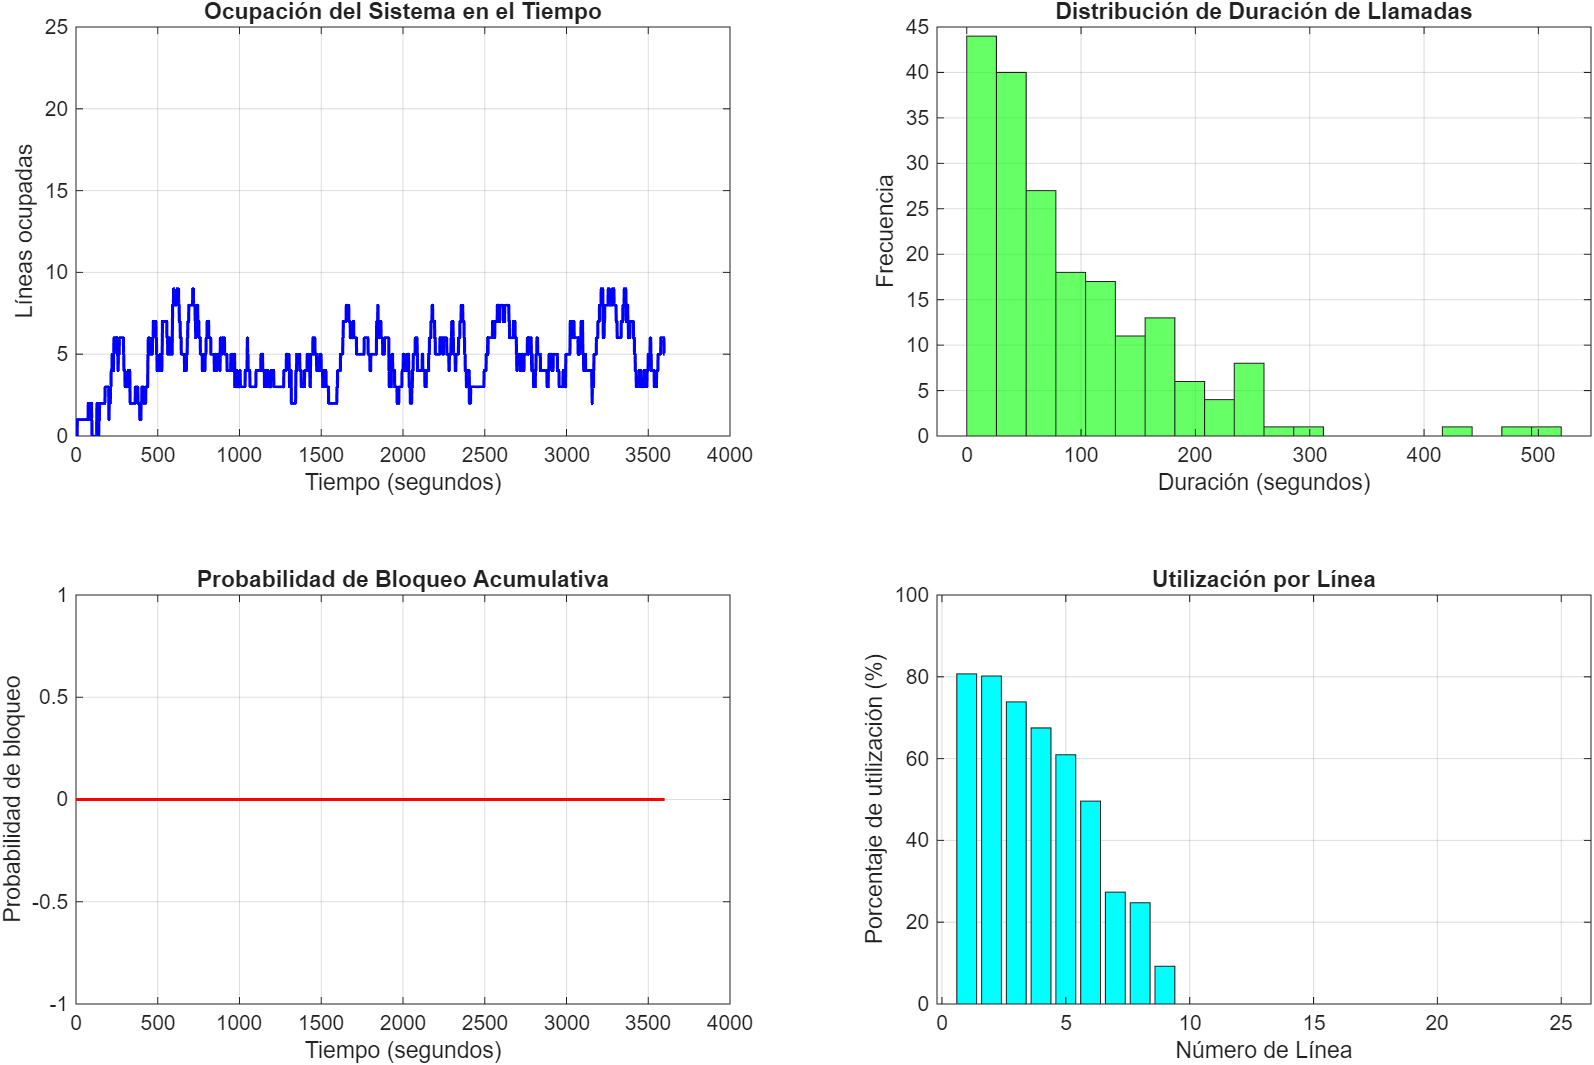
\includegraphics[width=0.8\columnwidth]{Figure_1.png}}
     \caption{ Ocupación del sistema en el tiempo.}
     \label{fig}
 \end{figure}

\subsection{Análisis de Tonos DTMF}\label{AA}
% insertar un parrafo
La figura 1 muestra la forma de onda de la señal DTMF para el dígito '5' en el dominio del tiempo. Se observa una señal periódica compleja, resultado de la suma de dos sinusoides.
% \begin{figure}[H]
%     \centerline{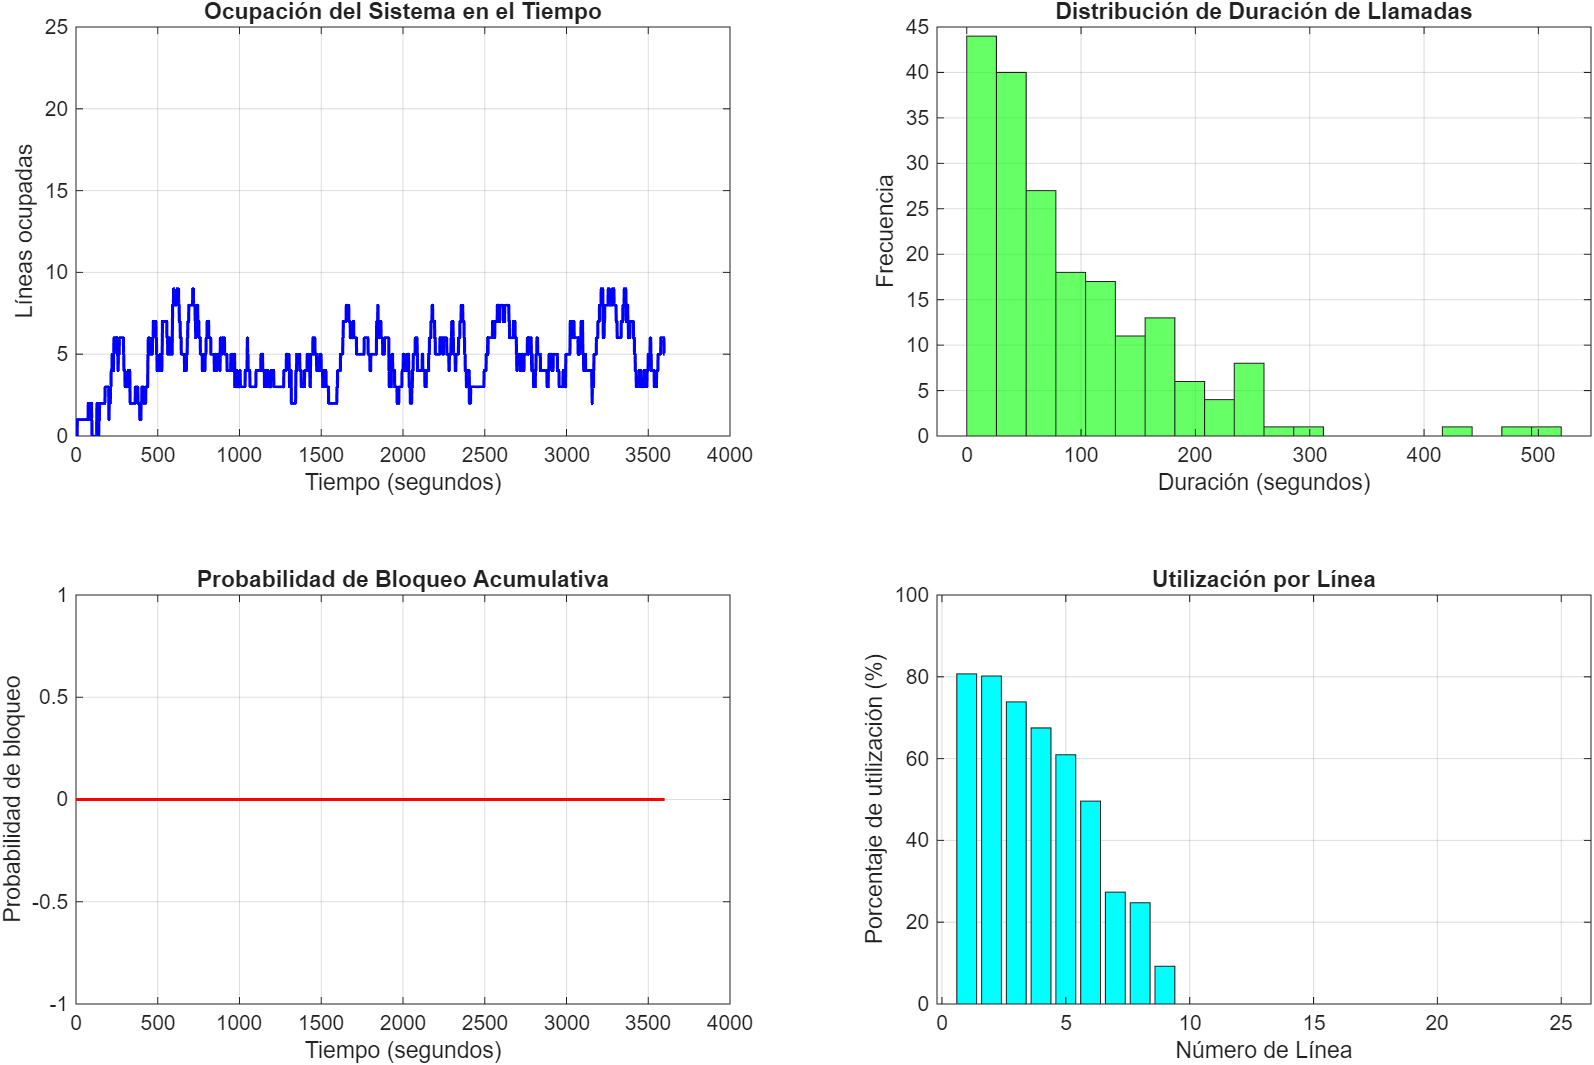
\includegraphics[width=0.8\columnwidth]{Figure_1.png}}
%     \caption{Forma de onda DTMF para el dígito '5'.}
%     \label{fig}
% \end{figure}

% %este texto tiene que estar despues de la fig 1 y antes de la fig 2

% La figura 2 muestra el espectro de frecuencias de la señal DTMF para el dígito '5'. Se identifican claramente los picos en las frecuencias correspondientes a 770 Hz y 1336 Hz, confirmando la composición dual-tone de la señal.

% \begin{figure}[H]
%     \centerline{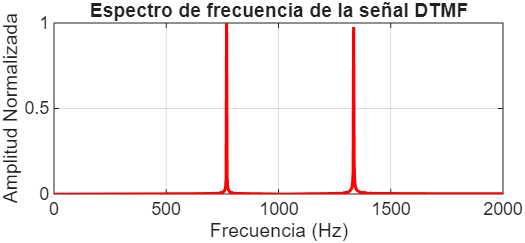
\includegraphics[width=0.8\columnwidth]{Figure_2.png}}
%     \caption{Espectro de frecuencias DTMF para el dígito '5'.}
%     \label{fig}
% \end{figure}

% La figura 3 muestra la forma de onda de la señal DTMF para el dígito '1' en el dominio del tiempo. Se observa una señal periódica compleja, resultado de la suma de dos sinusoides.

% \begin{figure}[H]
%     \centerline{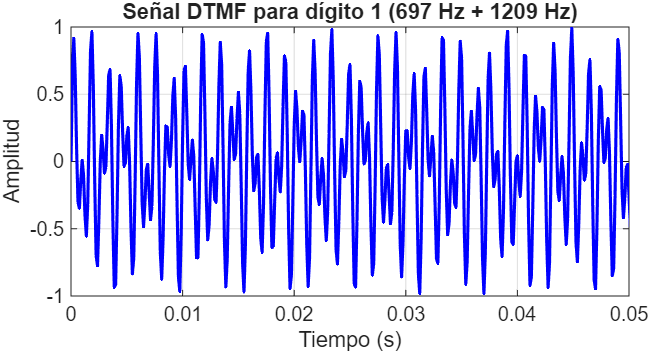
\includegraphics[width=0.8\columnwidth]{Figure_3.png}}
%     \caption{Forma de onda DTMF para el dígito '1'.}
%     \label{fig}
% \end{figure}


% La figura 4 muestra el espectro de frecuencias de la señal DTMF para el dígito '1'. Se identifican claramente los picos en las frecuencias correspondientes a 697 Hz y 1209 Hz, confirmando la composición dual-tone de la señal.
% \begin{figure}[H]
%     \centerline{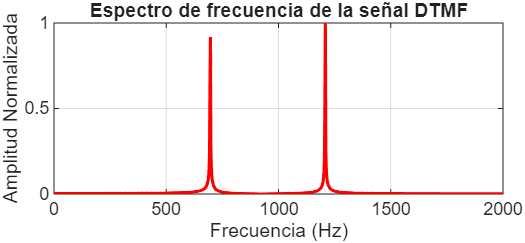
\includegraphics[width=0.8\columnwidth]{Figure_4.png}}
%     \caption{Espectro de frecuencias DTMF para el dígito '1'.}
%     \label{fig}
% \end{figure}


% La figura 5 muestra la forma de onda de la señal DTMF para el dígito 'C' en el dominio del tiempo. Se observa una señal periódica compleja, resultado de la suma de dos sinusoides.
% \begin{figure}[H]
%     \centerline{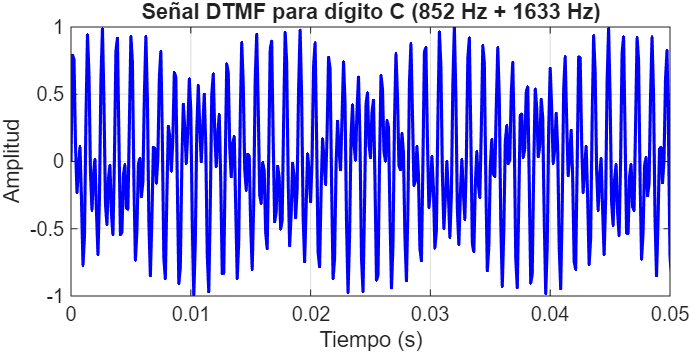
\includegraphics[width=0.8\columnwidth]{Figure_5.png}}
%     \caption{Forma de onda DTMF para el dígito 'C'.}
%     \label{fig}
% \end{figure}


% La figura 6 muestra el espectro de frecuencias de la señal DTMF para el dígito 'C'. Se identifican claramente los picos en las frecuencias correspondientes a 852 Hz y 1477 Hz, confirmando la composición dual-tone de la señal.
% \begin{figure}[H]
%     \centerline{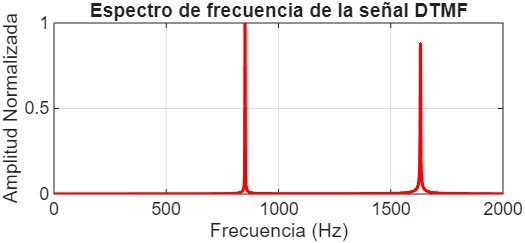
\includegraphics[width=0.8\columnwidth]{Figure_6.png}}
%     \caption{Espectro de frecuencias DTMF para el dígito 'C'.}
%     \label{fig} 
% \end{figure}


% \subsection{Modulación PCM y Codificación de Voz}
% Creacion del archivo de audio voz\_prueba.wav con una señal de voz sintetica.
% \begin{verbatim}
%     === GRABADORA DE VOZ ===
% Frecuencia: 8000 Hz
% Duración: 5 segundos
% Archivo: voz_prueba.wav

% Preparando grabación...
% Grabando durante 5 segundos...
% HABLE AHORA...
% Grabación completada.
% Archivo guardado: voz_prueba.wav
% Duración: 5.00 segundos
% Muestras: 40000
% Error al guardar el archivo: Unrecognized field name "FileSize".

% ¿Reproducir grabación? (s/n): s
% Reproduciendo...

% === PROCESO COMPLETADO ===
% El archivo voz_prueba.wav está listo para usar.

% \end{verbatim}

% MODULACIÓN PCM Y CODIFICACIÓN DE VOZ
% \begin{verbatim}
%     El archivo voz_prueba.wav está listo para usar.
% SNQ PCM Uniforme 8-bit: 39.88 dB
% SNQ PCM + Companding A-law 8-bit: -3.09 dB
% Reproduciendo voz original...
% Reproduciendo voz con PCM uniforme 8-bit...
% Reproduciendo voz con companding A-law...

% --- CALIDAD DE VOZ ESTIMADA ---
% PCM Uniforme 8-bit: MOS = 4.5
% PCM + Companding: MOS = 2.5
% >> parte2
% SNQ PCM Uniforme 8-bit: 39.88 dB
% SNQ PCM + Companding A-law 8-bit: -3.09 dB
% Reproduciendo voz original...
% Reproduciendo voz con PCM uniforme 8-bit...
% Reproduciendo voz con companding A-law...

% --- CALIDAD DE VOZ ESTIMADA ---
% PCM Uniforme 8-bit: MOS = 4.5
% PCM + Companding: MOS = 2.5
% >> 

% \end{verbatim}

% La figura 7 muestra PCM uniforme con 4, 8 y 12 bits respectivamente. Se observa que a medida que aumenta la cantidad de bits, la señal cuantizada se aproxima más a la señal original, reduciendo el error de cuantización.
% % \begin{figure}[H]
%     \centerline{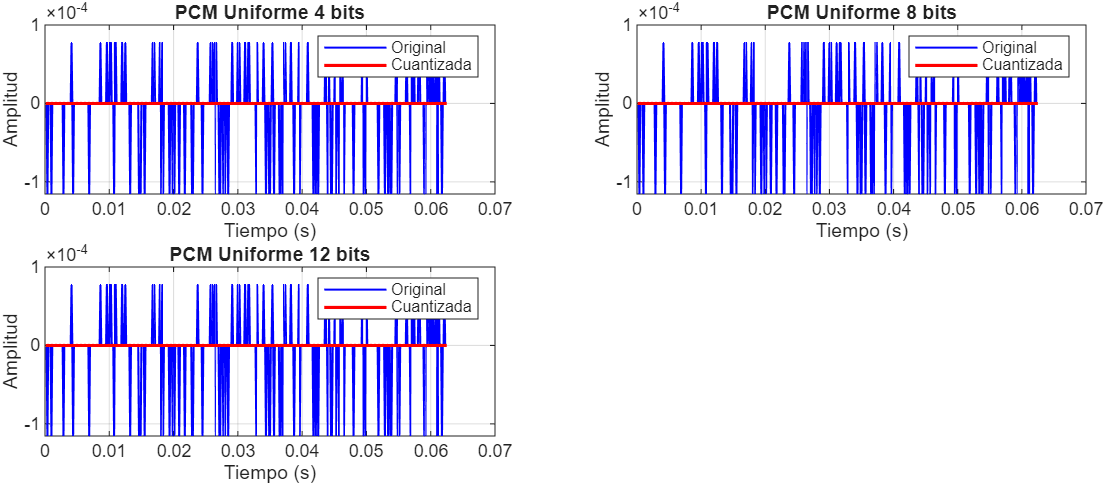
\includegraphics[width=0.8\columnwidth]{Figure_7.png}}
%     \caption{PCM uniforme con 4, 8 y 12 bits.}
%     \label{fig} 
% \end{figure}

% La figura 8 muestra Especro voz original, espectro PCM uniforme 8 bits, espectro error de cuantización y espectro PCM + companding A -law. Se observa que la PCM con companding A-law presenta un espectro más cercano al de la señal original, indicando una mejor preservación de las características de la voz.
% \begin{figure}[H]
%     \centerline{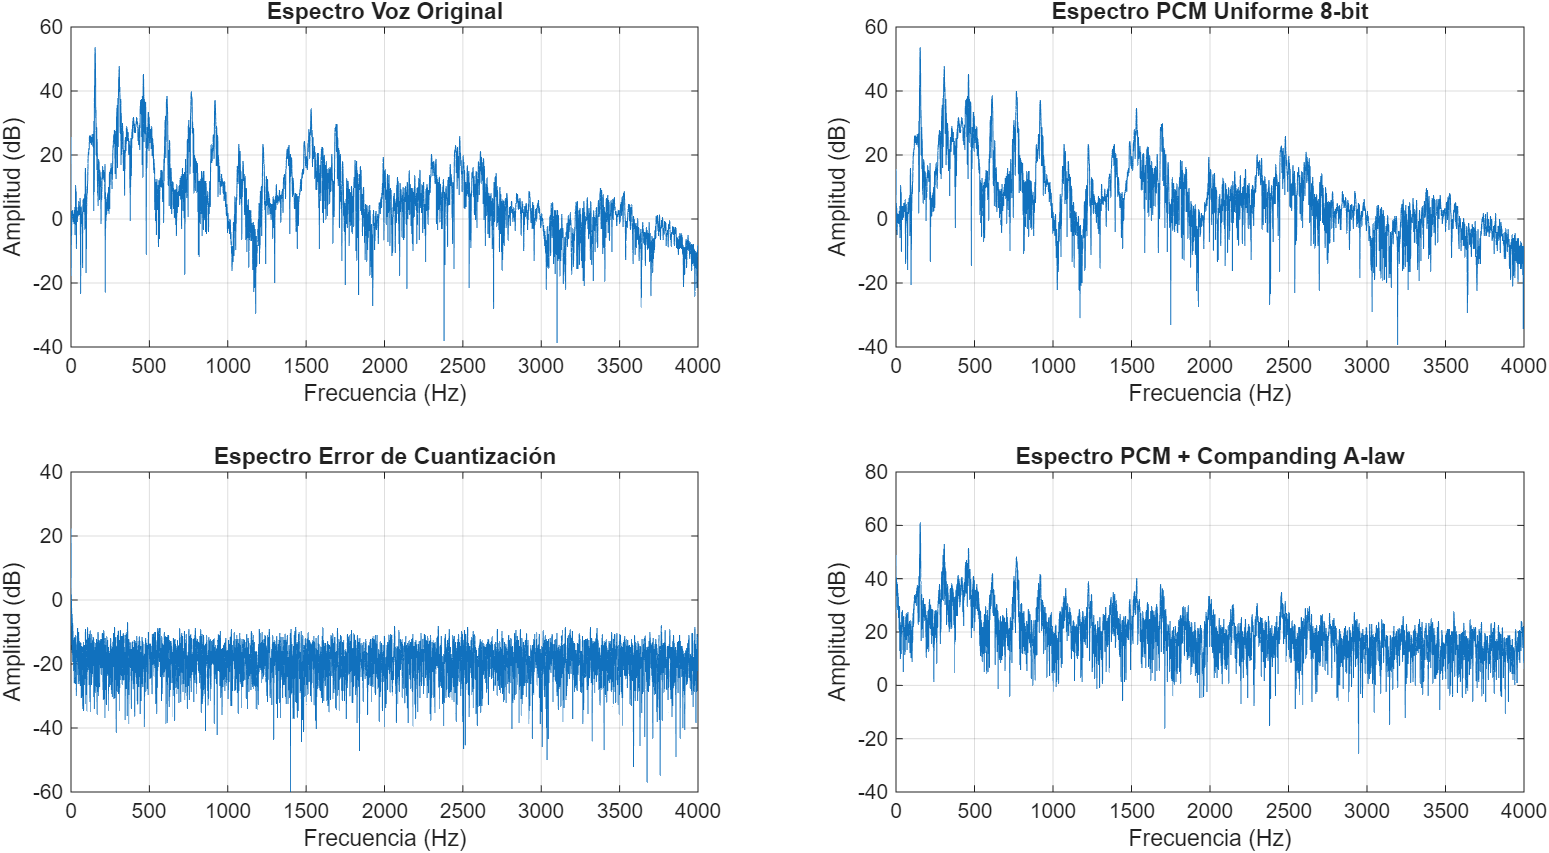
\includegraphics[width=0.8\columnwidth]{Figure_8.png}}
%     \caption{Espectros de voz original, PCM uniforme 8 bits, error de cuantización y PCM + companding A-law.}
%     \label{fig} 
% \end{figure}








\section{Conclusiones}

% \begin{itemize}
%     \item Se comprobó que la señalización DTMF funciona mediante la combinación de dos frecuencias específicas, lo que permite identificar de manera única cada dígito telefónico.
    
%     \item En la modulación PCM, se verificó que el número de bits de cuantización influye directamente en la calidad de la señal digitalizada: a mayor número de bits, menor error y mejor calidad de voz.
    
%     \item El uso de técnicas de companding (Ley A o Ley $\mu$) mejora la relación señal/ruido de cuantización y permite obtener una mejor calidad percibida sin necesidad de incrementar el número de bits.
    
%     \item Se comprobó que la elección de la frecuencia de muestreo ($f_s$) es crítica para evitar aliasing. Esto confirma lo establecido por el teorema de Nyquist-Shannon, que asegura una reconstrucción fiel de la señal cuando $f_s \geq 2f_{max}$.
    
%     \item El laboratorio permitió comprender de manera práctica cómo los procesos de muestreo y cuantización influyen directamente en la calidad del audio digital. Se comprobó que una reducción en el número de bits de cuantización genera un incremento en el error y en la distorsión de la señal, afectando la fidelidad de la voz y su inteligibilidad.
% \end{itemize}



% \section*{Acknowledgment}

% The preferred spelling of the word ``acknowledgment'' in America is without
% an ``e'' after the ``g''. Avoid the stilted expression ``one of us (R. B.
% G.) thanks $\ldots$''. Instead, try ``R. B. G. thanks$\ldots$''. Put sponsor
% acknowledgments in the unnumbered footnote on the first page.

% \section*{References}

% Please number citations consecutively within brackets \cite{b1}. The
% sentence punctuation follows the bracket \cite{b2}. Refer simply to the reference
% number, as in \cite{b3}---do not use ``Ref. \cite{b3}'' or ``reference \cite{b3}'' except at
% the beginning of a sentence: ``Reference \cite{b3} was the first $\ldots$''

% Number footnotes separately in superscripts. Place the actual footnote at
% the bottom of the column in which it was cited. Do not put footnotes in the
% abstract or reference list. Use letters for table footnotes.

% Unless there are six authors or more give all authors' names; do not use
% ``et al.''. Papers that have not been published, even if they have been
% submitted for publication, should be cited as ``unpublished'' \cite{b4}. Papers
% that have been accepted for publication should be cited as ``in press'' \cite{b5}.
% Capitalize only the first word in a paper title, except for proper nouns and
% element symbols.

% For papers published in translation journals, please give the English
% citation first, followed by the original foreign-language citation \cite{b6}.

\begin{thebibliography}{00}
    \bibitem{b1} IEEE, ``IEEE Conference Templates,'' [En línea]. Disponible en: https://www.ieee.org/conferences/publishing/templates. [Accedido: 16 sep. 2025].
    \bibitem{b2} MathWorks, ``MATLAB Graphics Documentation,'' [En línea]. Disponible en: https://la.mathworks.com/help/matlab/graphics.html. [Accedido: 16 sep. 2025].
    \bibitem{b3} Anthropic, ``Claude AI Assistant,'' [En línea]. Disponible en: https://claude.ai. [Accedido: 16 sep. 2025].
\end{thebibliography}
\vspace{12pt}
% \color{red}
% IEEE conference templates contain guidance text for composing and formatting conference papers. Please ensure that all template text is removed from your conference paper prior to submission to the conference. Failure to remove the template text from your paper may result in your paper not being published.

\end{document}
